% Options for packages loaded elsewhere
\PassOptionsToPackage{unicode}{hyperref}
\PassOptionsToPackage{hyphens}{url}
%
\documentclass[
]{article}
\usepackage{amsmath,amssymb}
\usepackage{iftex}
\ifPDFTeX
  \usepackage[T1]{fontenc}
  \usepackage[utf8]{inputenc}
  \usepackage{textcomp} % provide euro and other symbols
\else % if luatex or xetex
  \usepackage{unicode-math} % this also loads fontspec
  \defaultfontfeatures{Scale=MatchLowercase}
  \defaultfontfeatures[\rmfamily]{Ligatures=TeX,Scale=1}
\fi
\usepackage{lmodern}
\ifPDFTeX\else
  % xetex/luatex font selection
\fi
% Use upquote if available, for straight quotes in verbatim environments
\IfFileExists{upquote.sty}{\usepackage{upquote}}{}
\IfFileExists{microtype.sty}{% use microtype if available
  \usepackage[]{microtype}
  \UseMicrotypeSet[protrusion]{basicmath} % disable protrusion for tt fonts
}{}
\makeatletter
\@ifundefined{KOMAClassName}{% if non-KOMA class
  \IfFileExists{parskip.sty}{%
    \usepackage{parskip}
  }{% else
    \setlength{\parindent}{0pt}
    \setlength{\parskip}{6pt plus 2pt minus 1pt}}
}{% if KOMA class
  \KOMAoptions{parskip=half}}
\makeatother
\usepackage{xcolor}
\usepackage[margin=1in]{geometry}
\usepackage{color}
\usepackage{fancyvrb}
\newcommand{\VerbBar}{|}
\newcommand{\VERB}{\Verb[commandchars=\\\{\}]}
\DefineVerbatimEnvironment{Highlighting}{Verbatim}{commandchars=\\\{\}}
% Add ',fontsize=\small' for more characters per line
\usepackage{framed}
\definecolor{shadecolor}{RGB}{248,248,248}
\newenvironment{Shaded}{\begin{snugshade}}{\end{snugshade}}
\newcommand{\AlertTok}[1]{\textcolor[rgb]{0.94,0.16,0.16}{#1}}
\newcommand{\AnnotationTok}[1]{\textcolor[rgb]{0.56,0.35,0.01}{\textbf{\textit{#1}}}}
\newcommand{\AttributeTok}[1]{\textcolor[rgb]{0.13,0.29,0.53}{#1}}
\newcommand{\BaseNTok}[1]{\textcolor[rgb]{0.00,0.00,0.81}{#1}}
\newcommand{\BuiltInTok}[1]{#1}
\newcommand{\CharTok}[1]{\textcolor[rgb]{0.31,0.60,0.02}{#1}}
\newcommand{\CommentTok}[1]{\textcolor[rgb]{0.56,0.35,0.01}{\textit{#1}}}
\newcommand{\CommentVarTok}[1]{\textcolor[rgb]{0.56,0.35,0.01}{\textbf{\textit{#1}}}}
\newcommand{\ConstantTok}[1]{\textcolor[rgb]{0.56,0.35,0.01}{#1}}
\newcommand{\ControlFlowTok}[1]{\textcolor[rgb]{0.13,0.29,0.53}{\textbf{#1}}}
\newcommand{\DataTypeTok}[1]{\textcolor[rgb]{0.13,0.29,0.53}{#1}}
\newcommand{\DecValTok}[1]{\textcolor[rgb]{0.00,0.00,0.81}{#1}}
\newcommand{\DocumentationTok}[1]{\textcolor[rgb]{0.56,0.35,0.01}{\textbf{\textit{#1}}}}
\newcommand{\ErrorTok}[1]{\textcolor[rgb]{0.64,0.00,0.00}{\textbf{#1}}}
\newcommand{\ExtensionTok}[1]{#1}
\newcommand{\FloatTok}[1]{\textcolor[rgb]{0.00,0.00,0.81}{#1}}
\newcommand{\FunctionTok}[1]{\textcolor[rgb]{0.13,0.29,0.53}{\textbf{#1}}}
\newcommand{\ImportTok}[1]{#1}
\newcommand{\InformationTok}[1]{\textcolor[rgb]{0.56,0.35,0.01}{\textbf{\textit{#1}}}}
\newcommand{\KeywordTok}[1]{\textcolor[rgb]{0.13,0.29,0.53}{\textbf{#1}}}
\newcommand{\NormalTok}[1]{#1}
\newcommand{\OperatorTok}[1]{\textcolor[rgb]{0.81,0.36,0.00}{\textbf{#1}}}
\newcommand{\OtherTok}[1]{\textcolor[rgb]{0.56,0.35,0.01}{#1}}
\newcommand{\PreprocessorTok}[1]{\textcolor[rgb]{0.56,0.35,0.01}{\textit{#1}}}
\newcommand{\RegionMarkerTok}[1]{#1}
\newcommand{\SpecialCharTok}[1]{\textcolor[rgb]{0.81,0.36,0.00}{\textbf{#1}}}
\newcommand{\SpecialStringTok}[1]{\textcolor[rgb]{0.31,0.60,0.02}{#1}}
\newcommand{\StringTok}[1]{\textcolor[rgb]{0.31,0.60,0.02}{#1}}
\newcommand{\VariableTok}[1]{\textcolor[rgb]{0.00,0.00,0.00}{#1}}
\newcommand{\VerbatimStringTok}[1]{\textcolor[rgb]{0.31,0.60,0.02}{#1}}
\newcommand{\WarningTok}[1]{\textcolor[rgb]{0.56,0.35,0.01}{\textbf{\textit{#1}}}}
\usepackage{graphicx}
\makeatletter
\newsavebox\pandoc@box
\newcommand*\pandocbounded[1]{% scales image to fit in text height/width
  \sbox\pandoc@box{#1}%
  \Gscale@div\@tempa{\textheight}{\dimexpr\ht\pandoc@box+\dp\pandoc@box\relax}%
  \Gscale@div\@tempb{\linewidth}{\wd\pandoc@box}%
  \ifdim\@tempb\p@<\@tempa\p@\let\@tempa\@tempb\fi% select the smaller of both
  \ifdim\@tempa\p@<\p@\scalebox{\@tempa}{\usebox\pandoc@box}%
  \else\usebox{\pandoc@box}%
  \fi%
}
% Set default figure placement to htbp
\def\fps@figure{htbp}
\makeatother
\setlength{\emergencystretch}{3em} % prevent overfull lines
\providecommand{\tightlist}{%
  \setlength{\itemsep}{0pt}\setlength{\parskip}{0pt}}
\setcounter{secnumdepth}{-\maxdimen} % remove section numbering
\usepackage{bookmark}
\IfFileExists{xurl.sty}{\usepackage{xurl}}{} % add URL line breaks if available
\urlstyle{same}
\hypersetup{
  pdftitle={Untitled},
  pdfauthor={250539-PCA-Next-Step},
  hidelinks,
  pdfcreator={LaTeX via pandoc}}

\title{Untitled}
\author{250539-PCA-Next-Step}
\date{2025-05-30}

\begin{document}
\maketitle

\subsection{Key Questions}\label{key-questions}

\begin{enumerate}
\def\labelenumi{\arabic{enumi}.}
\tightlist
\item
  What data preprocessing can work on methylation data? Do we need to
  scale it or row center it? This is essential to feature selection.
\item
  What dimension reduction method should we choose? What modification of
  PCA should we choose?
\item
  If we want to compare graphs of important gene networks, what summary
  features should we choose to reduce computational complexity? How to
  measure them? (far away, after important genes are filtered out)
\end{enumerate}

\subsection{Next Step}\label{next-step}

\begin{enumerate}
\def\labelenumi{\arabic{enumi}.}
\tightlist
\item
  Unify bin size of the methylation distribution graphs
\item
  Literature search for dimensional reduction on hyper and hypo
  methylation, PCA can only find important features by very large
  absolute values, not by values near 0.
\item
  Mathematical explanation on why only negative values show up in PC 1,
  further investigate relationship between \(\bf v_1\) and \(\bf u_1\),
  beyond matrix multiplication of \(C_p\)
\item
  Read neuroscience paper recommended by Elena and self-teach graph
  properties.
\item
  Generalized results and simulations for non-negative matrix singular
  vector signs.
\end{enumerate}

\subsection{1. How to interprete the DNA mathylation
dataset?}\label{how-to-interprete-the-dna-mathylation-dataset}

Raw methylation was quantified as methylation counts of base pairs in
consecutive 300 base pair (bp) intervals across the genome. Then,
ComBat-Seq was applied to remove batch effect, and DESeq2 was applied to
normalize the batch-corrected counts.

In the supplementary matrials, the link to the source code is attached:
\pandocbounded{\includegraphics[keepaspectratio]{https://github.com/HansenHeLab/cfMeDIP-seq_Data_Resource_Codes/blob/main/1_Methylation_Scripts/R_scripts_to_process_features/4.2_Batch_correction_for_SE_PE.R}}

The image below shows that \texttt{Combat\_seq} assumes that the raw
methylation count data follows a negative binomial distribution:
\(NB(\mu_{gij}, \phi_{gi})\), where \(\mu_{gij}, \phi_{gi}\) are the
mean and dispersion parameter. The log mean count of gene g in batch i
and sample j is linearly modelled by

\begin{enumerate}
\def\labelenumi{\arabic{enumi}.}
\tightlist
\item
  \(\alpha_g\): The overall the level of gene g
\item
  \(X_j\): The biological condition of sample j
\item
  \(\beta_g\): The regression cofficient for the gene g
\item
  \(\gamma_{gi}\): The mean match effect of batch i and gene j
\item
  \(N_j\): The total count of all genes in sample j
\end{enumerate}

The mean value of the batch-free distribution is estimated. Every
\(y_{gij}\) in the empirical distribution is mapped to the closest
quantile in the batch free distribution. Since NB distribution is
integer valued, the quantile mapped to will also be an integer.

\pandocbounded{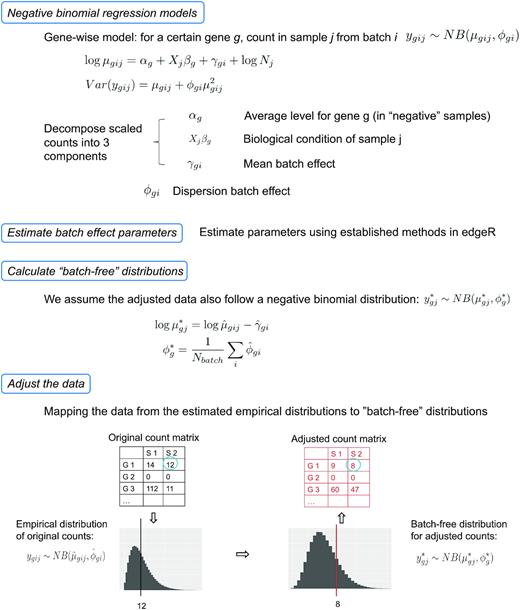
\includegraphics[keepaspectratio]{../Images/ComBat-seq.jpeg}}
Source:
\pandocbounded{\includegraphics[keepaspectratio]{https://academic.oup.com/nargab/article/2/3/lqaa078/5909519}}

The batch-corrected values can be proportional to both the actual
methylation of DNA and many other uninteresting factors such as 1)
Sequencing depth of genes in different samples 2) gene length 3) RNA
composition.

DESeq2 adjust the methylation scores by both sequencing depth and RNA
composition. DESeq2 applies a median of ratios method in following
steps:

\begin{enumerate}
\def\labelenumi{\arabic{enumi}.}
\tightlist
\item
  Create a psuedo-reference sample: by computing the geometric mean of
  each gene across samples. Such geometric means will be used as a
  reference.
\item
  Ratio of sample to the reference: for each gene, divide the
  methylation different sample by the corresponding the
  pseudo-reference.
\item
  Calcuate the normalization factor for each sample: for each given
  sample, find the median of all ratios, such a median will be used as
  the normalization factor, or the size factor.
\item
  Normalize the count: divide each count value in a given sample by that
  sample's normalization factor. Integer valued methylation will become
  decimal in this step.
\end{enumerate}

``This method is robust to imbalance in up-/down-regulation and large
numbers of differentially expressed genes.''

Source:
\pandocbounded{\includegraphics[keepaspectratio]{https://hbctraining.github.io/DGE_workshop/lessons/02_DGE_count_normalization.html}}

\subsection{2. Simulation: is the first right singular vector always
negative?}\label{simulation-is-the-first-right-singular-vector-always-negative}

\begin{Shaded}
\begin{Highlighting}[]
\NormalTok{n }\OtherTok{\textless{}{-}} \DecValTok{10}
\NormalTok{p }\OtherTok{\textless{}{-}} \DecValTok{50}
\NormalTok{B }\OtherTok{\textless{}{-}} \DecValTok{200} \DocumentationTok{\#\# Simulate 100 times}
\NormalTok{allNegLeft.vec }\OtherTok{\textless{}{-}} \FunctionTok{c}\NormalTok{()}
\NormalTok{allNegRight.vec }\OtherTok{\textless{}{-}} \FunctionTok{c}\NormalTok{()}


\ControlFlowTok{for}\NormalTok{ (b }\ControlFlowTok{in} \DecValTok{1}\SpecialCharTok{:}\NormalTok{B) \{}
\NormalTok{  X }\OtherTok{\textless{}{-}} \FunctionTok{rexp}\NormalTok{(n}\SpecialCharTok{*}\NormalTok{p, }\DecValTok{3}\NormalTok{)}
\NormalTok{  X }\OtherTok{\textless{}{-}} \FunctionTok{matrix}\NormalTok{(X, }\AttributeTok{nrow =}\NormalTok{ n, }\AttributeTok{ncol =}\NormalTok{ p)}
  
\NormalTok{  svdRes }\OtherTok{\textless{}{-}} \FunctionTok{svd}\NormalTok{(X)}
\NormalTok{  u1 }\OtherTok{\textless{}{-}}\NormalTok{ svdRes}\SpecialCharTok{$}\NormalTok{u[,}\DecValTok{1}\NormalTok{]}
\NormalTok{  v1 }\OtherTok{\textless{}{-}}\NormalTok{ svdRes}\SpecialCharTok{$}\NormalTok{v[,}\DecValTok{1}\NormalTok{]}
  
  \CommentTok{\# print(svdRes$d)}
\NormalTok{  allNegLeft.vec }\OtherTok{\textless{}{-}} \FunctionTok{c}\NormalTok{(allNegLeft.vec, }\FunctionTok{all}\NormalTok{(v1 }\SpecialCharTok{\textless{}} \DecValTok{0}\NormalTok{))}
\NormalTok{  allNegRight.vec }\OtherTok{\textless{}{-}} \FunctionTok{c}\NormalTok{(allNegRight.vec, }\FunctionTok{all}\NormalTok{(u1 }\SpecialCharTok{\textless{}} \DecValTok{0}\NormalTok{))}
\NormalTok{\}}

\FunctionTok{cat}\NormalTok{(}\StringTok{"Times that all v1 elements are negative:"}\NormalTok{, }\FunctionTok{sum}\NormalTok{(allNegRight.vec), }\StringTok{"}\SpecialCharTok{\textbackslash{}n}\StringTok{"}\NormalTok{)}
\end{Highlighting}
\end{Shaded}

\begin{verbatim}
## Times that all v1 elements are negative: 200
\end{verbatim}

\begin{Shaded}
\begin{Highlighting}[]
\FunctionTok{cat}\NormalTok{(}\StringTok{"Times that all u1 elements are negative:"}\NormalTok{, }\FunctionTok{sum}\NormalTok{(allNegLeft.vec))}
\end{Highlighting}
\end{Shaded}

\begin{verbatim}
## Times that all u1 elements are negative: 200
\end{verbatim}

Observation: the top right singular vector is always negative in the
simulation. Left singular vectors are negative as well.

Question: what if one of the singular values of \(X^T X\) is negative,
how is the corresponding singular vector adjusted accordingly?

\begin{Shaded}
\begin{Highlighting}[]
\DocumentationTok{\#\# Simulation: generate the left and right singular matrices}
\NormalTok{U }\OtherTok{\textless{}{-}}\NormalTok{ svdRes}\SpecialCharTok{$}\NormalTok{u}
\NormalTok{V }\OtherTok{\textless{}{-}}\NormalTok{ svdRes}\SpecialCharTok{$}\NormalTok{v}
\NormalTok{D }\OtherTok{\textless{}{-}} \FunctionTok{diag}\NormalTok{(}\FunctionTok{c}\NormalTok{(}\DecValTok{5}\NormalTok{,}\SpecialCharTok{{-}}\DecValTok{5}\NormalTok{, }\DecValTok{0}\NormalTok{,}\DecValTok{0}\NormalTok{,}\DecValTok{0}\NormalTok{,}\DecValTok{0}\NormalTok{,}\DecValTok{0}\NormalTok{,}\DecValTok{0}\NormalTok{,}\DecValTok{0}\NormalTok{,}\DecValTok{0}\NormalTok{))}

\NormalTok{Z }\OtherTok{\textless{}{-}}\NormalTok{ U }\SpecialCharTok{\%*\%}\NormalTok{ D }\SpecialCharTok{\%*\%} \FunctionTok{t}\NormalTok{(V)}
\NormalTok{Z.svdRes }\OtherTok{\textless{}{-}} \FunctionTok{svd}\NormalTok{(Z)}
\FunctionTok{plot}\NormalTok{(Z.svdRes}\SpecialCharTok{$}\NormalTok{d)}
\end{Highlighting}
\end{Shaded}

\pandocbounded{\includegraphics[keepaspectratio]{250530-PCA-Next-Step_files/figure-latex/unnamed-chunk-2-1.pdf}}

\begin{Shaded}
\begin{Highlighting}[]
\FunctionTok{heatmap}\NormalTok{(}\FunctionTok{t}\NormalTok{(}\FunctionTok{sign}\NormalTok{(Z.svdRes}\SpecialCharTok{$}\NormalTok{v)))}
\end{Highlighting}
\end{Shaded}

\pandocbounded{\includegraphics[keepaspectratio]{250530-PCA-Next-Step_files/figure-latex/unnamed-chunk-2-2.pdf}}
Observation: true singular values of the same absolute values repeated
themselves in the estimated singular value list. This means if that the
construction of the data matrix contains negative weight, they will be
masked by the positive version during the SVD of the target matrix.

\begin{Shaded}
\begin{Highlighting}[]
\CommentTok{\# seCount.svd \textless{}{-} svd(seCount)}
\CommentTok{\# plot(seCount.svd$d[1:20], type = "l")}
\CommentTok{\# }
\CommentTok{\# heatmap(sign(seCount.svd$u[1:50, 1:20]))}
\end{Highlighting}
\end{Shaded}

\subsection{3. Sample centering: the relationship between right singular
vector in the original matrix and in the row-centred (sample-centred)
matrix}\label{sample-centering-the-relationship-between-right-singular-vector-in-the-original-matrix-and-in-the-row-centred-sample-centred-matrix}

Treating every sample of the mathylation matrix as a row, before the row
centering, finding the top PC is equivalent to solving the following
optimization problem: \[
\text{max } \{\bf v_1^T S \bf{v_1} \} \text{   s.t   } \|v_1 \|_2 = 1
\]

where \(S = \frac{1}{n-1} X^T C_n X\), and \(C_n\) is the column
centering operator.

After row-centering, the optimization becomes: \[
\text{max } \{\bf w_1^T (\frac{1}{n-1} C_p X^T C_n X C_p) \bf{w_1} \} \text{   s.t   } \|w_1 \|_2 = 1
\] Let \(\bf{u_1} = C_p \bf{w_1}\), the problem can be reformulated as
\[
\text{max } \{\bf{u_1}^t (\frac{1}{n-1} X^T C_n X) \bf{u_1} \} \text{   s.t   } \|\bf{u_1} \|_2 = 1 - \bar{v}^2
\] where \(\bar{v}\) is the average value of elements in the first PC.

The Lagarangian is:

\[
L(\bf{u_1}, \lambda) = \bf{u_1}^t S \bf{u_1} + \lambda*(1 - \bar{v}^2 - \bf{u_1}^T \bf{u_1})
\] Taking partial derivatives and setting to 0: \[
\frac{\partial L}{\partial \bf{u_1}} = 2 S \bf{u_1} - 2\lambda*\bf{u_1} = 0
\] \[
\frac{\partial L}{\partial \lambda} = 1 - \bar{v}^2 - \bf{u_1}^T \bf{u_1} = 0
\]

\begin{enumerate}
\def\labelenumi{\arabic{enumi}.}
\tightlist
\item
  Let \(\bf{v_1}^*\) and \(\bf{u_1}^*\) be the solution to the
  maximization problem before and after row-centering.
  \(\frac{\partial L}{\partial \bf{u_1}} = 0\) suggests that
  \(\bf{u_1}^*\) is the first eigenvalue of S, so
  \(\bf{u_1}^* = K \bf{v_1}^*\) for some constant K. And since
  \(\bf{u_1}^* = C_p \bf{w_1}^*\), this implies that
  \(\frac{1}{K} C_p \bf{w_1}^* = \bf{v_1}^*\).
\item
  \(\frac{\partial L}{\partial \lambda} = 0\) suggests that the
  \(\bf{u_1}\) is the unit vector \(\bf{v_1}\) scaled by
  \(\sqrt{1 - \bar{v}^2}\):
  \(\bf{u_1} = \frac{\bf{v_1}}{\sqrt{1 - \bar{v}^2}}\). Therefore,
  \(K = \frac{1}{\sqrt{1 - \bar{v}^2}}\)
\end{enumerate}

So, putting everything together,

\[
C_p \bf{w_1}^* \sqrt{1 - \bar{v}^2} = \bf{v_1}^*
\]

\begin{Shaded}
\begin{Highlighting}[]
\DocumentationTok{\#\# Simulation}
\NormalTok{n }\OtherTok{\textless{}{-}} \DecValTok{20} \DocumentationTok{\#\# rows for genes}
\NormalTok{p }\OtherTok{\textless{}{-}} \DecValTok{10} \DocumentationTok{\#\# columns for samples}

\DocumentationTok{\#\# L2 norm}
\NormalTok{norm }\OtherTok{\textless{}{-}} \ControlFlowTok{function}\NormalTok{(x) \{}
  \FunctionTok{sqrt}\NormalTok{(}\FunctionTok{sum}\NormalTok{(x}\SpecialCharTok{\^{}}\DecValTok{2}\NormalTok{))}
\NormalTok{\}}

\DocumentationTok{\#\# Before row{-}centering}
\NormalTok{X }\OtherTok{\textless{}{-}} \FunctionTok{rexp}\NormalTok{(n}\SpecialCharTok{*}\NormalTok{p, }\DecValTok{3}\NormalTok{)}
\NormalTok{X }\OtherTok{\textless{}{-}} \FunctionTok{matrix}\NormalTok{(X, }\AttributeTok{nrow =}\NormalTok{ n, }\AttributeTok{ncol =}\NormalTok{ p)}
\NormalTok{X.svd }\OtherTok{\textless{}{-}} \FunctionTok{svd}\NormalTok{(X)}
\NormalTok{v1 }\OtherTok{\textless{}{-}}\NormalTok{ X.svd}\SpecialCharTok{$}\NormalTok{v[,}\DecValTok{1}\NormalTok{]}
\NormalTok{v1 }\OtherTok{\textless{}{-}}\NormalTok{ v1}\SpecialCharTok{/}\FunctionTok{norm}\NormalTok{(v1)}


\DocumentationTok{\#\# After row{-}centering}
\NormalTok{X.rc }\OtherTok{\textless{}{-}} \FunctionTok{t}\NormalTok{(}\FunctionTok{scale}\NormalTok{(}\FunctionTok{t}\NormalTok{(X), }\AttributeTok{center =}\NormalTok{ T))}
\NormalTok{X.rc.svd }\OtherTok{\textless{}{-}} \FunctionTok{svd}\NormalTok{(X.rc)}
\NormalTok{w1 }\OtherTok{\textless{}{-}}\NormalTok{ X.rc.svd}\SpecialCharTok{$}\NormalTok{v[,}\DecValTok{1}\NormalTok{]}
\NormalTok{w1 }\OtherTok{\textless{}{-}}\NormalTok{ u1}\SpecialCharTok{/}\FunctionTok{norm}\NormalTok{(u1)}


\DocumentationTok{\#\# Transformation:}
\NormalTok{v.bar }\OtherTok{\textless{}{-}} \FunctionTok{mean}\NormalTok{(v1)}
\NormalTok{K }\OtherTok{\textless{}{-}} \DecValTok{1}\SpecialCharTok{/}\FunctionTok{sqrt}\NormalTok{(}\DecValTok{1} \SpecialCharTok{{-}}\NormalTok{ v.bar}\SpecialCharTok{\^{}}\DecValTok{2}\NormalTok{)}
\NormalTok{C\_p }\OtherTok{=} \FunctionTok{diag}\NormalTok{(p) }\SpecialCharTok{{-}}  \FunctionTok{rep}\NormalTok{(}\DecValTok{1}\NormalTok{, p) }\SpecialCharTok{\%*\%} \FunctionTok{t}\NormalTok{(}\FunctionTok{rep}\NormalTok{(}\DecValTok{1}\NormalTok{, p)) }\SpecialCharTok{/}\NormalTok{ p}

\NormalTok{u1 }\OtherTok{\textless{}{-}}\NormalTok{ C\_p }\SpecialCharTok{\%*\%}\NormalTok{ w1}
\NormalTok{u1 }\SpecialCharTok{{-}}\NormalTok{ v1}\SpecialCharTok{*}\NormalTok{K}
\end{Highlighting}
\end{Shaded}

\begin{verbatim}
##            [,1]
##  [1,] 0.4011068
##  [2,] 0.3671625
##  [3,] 0.3768812
##  [4,] 0.3575770
##  [5,] 0.2810983
##  [6,] 0.3114972
##  [7,] 0.3131033
##  [8,] 0.1976419
##  [9,] 0.2181019
## [10,] 0.4633775
\end{verbatim}

\begin{Shaded}
\begin{Highlighting}[]
\FunctionTok{par}\NormalTok{(}\AttributeTok{mfrow =} \FunctionTok{c}\NormalTok{(}\DecValTok{2}\NormalTok{,}\DecValTok{1}\NormalTok{))}
\FunctionTok{plot}\NormalTok{(v1, }\AttributeTok{type =} \StringTok{"l"}\NormalTok{, }\AttributeTok{main =} \StringTok{"PC 1 before row{-}centering"}\NormalTok{)}
\FunctionTok{plot}\NormalTok{(u1, }\AttributeTok{type =} \StringTok{"l"}\NormalTok{, }\AttributeTok{main =} \StringTok{"PC 1 after row{-}centering"}\NormalTok{)}
\end{Highlighting}
\end{Shaded}

\pandocbounded{\includegraphics[keepaspectratio]{250530-PCA-Next-Step_files/figure-latex/unnamed-chunk-4-1.pdf}}

\begin{Shaded}
\begin{Highlighting}[]
\FunctionTok{plot}\NormalTok{(w1, }\AttributeTok{type =} \StringTok{"l"}\NormalTok{, }\AttributeTok{main =} \StringTok{"PC 1 before row{-}centering after transformation"}\NormalTok{)}
\end{Highlighting}
\end{Shaded}

\pandocbounded{\includegraphics[keepaspectratio]{250530-PCA-Next-Step_files/figure-latex/unnamed-chunk-4-2.pdf}}

\end{document}
